\documentclass[12pt, letterpaper]{article}
\usepackage[utf8]{inputenc}
\usepackage{newunicodechar}
\usepackage{pdfpages}
\usepackage{graphicx}
\documentstyle{article}

% Math-mode symbol & verbatim
\def\W#1#2{$#1{#2}$ &\tt\string#1\string{#2\string}}
\def\X#1{$#1$ &\tt\string#1}
\def\Y#1{$\big#1$ &\tt\string#1}
\def\Z#1{\tt\string#1}

% A non-floating table environment.
\makeatletter
\renewenvironment{table}%
   {\vskip\intextsep\parskip\z@
    \vbox\bgroup\centering\def\@captype{table}}%
   {\egroup\vskip\intextsep}
\makeatother

% All the tables are \label'ed in case this document ever gets some
% explanatory text written, however there are no \refs as yet. To save
% LaTeX-ing the file twice we go:
\renewcommand{\label}[1]{}

% A4 page setup
\topmargin -45pt
\textwidth=532pt
\oddsidemargin=-40pt \evensidemargin\oddsidemargin
\textheight 682pt

\begin{document}

\begin{table}
\begin{tabular}{*8l}
\X\alpha        &\X\theta       &\X o           &\X\tau         \\
\X\beta         &\X\vartheta    &\X\pi          &\X\upsilon     \\
\X\gamma        &\X\gamma       &\X\varpi       &\X\phi         \\
\X\delta        &\X\kappa       &\X\rho         &\X\varphi      \\
\X\epsilon      &\X\lambda      &\X\varrho      &\X\chi         \\
\X\varepsilon   &\X\mu          &\X\sigma       &\X\psi         \\
\X\zeta         &\X\nu          &\X\varsigma    &\X\omega       \\
\X\eta          &\X\xi                                          \\
                                                                \\
\X\Gamma        &\X\Lambda      &\X\Sigma       &\X\Psi         \\
\X\Delta        &\X\Xi          &\X\Upsilon     &\X\Omega       \\
\X\Theta        &\X\Pi          &\X\Phi
\end{tabular}
\caption{Greek Letters}\label{greek}
\end{table}

\begin{table}
\begin{tabular}{*8l}
\X\pm           &\X\cap         &\X\diamond             &\X\oplus     \\
\X\mp           &\X\cup         &\X\bigtriangleup       &\X\ominus    \\
\X\times        &\X\uplus       &\X\bigtriangledown     &\X\otimes    \\
\X\div          &\X\sqcap       &\X\triangleleft        &\X\oslash    \\
\X\ast          &\X\sqcup       &\X\triangleright       &\X\odot      \\
\X\star         &\X\vee         &\X\lhd$^b$             &\X\bigcirc   \\
\X\circ         &\X\wedge       &\X\rhd$^b$             &\X\dagger    \\
\X\bullet       &\X\setminus    &\X\unlhd$^b$           &\X\ddagger   \\
\X\cdot         &\X\wr          &\X\unrhd$^b$           &\X\amalg     \\
\X+             &\X-
\end{tabular}

$^b$ Not predefined in a format based on {\tt basefont.tex}.
     Use one of the style options\\
     {\tt oldlfont}, {\tt newlfont}, {\tt amsfonts} or {\tt amssymb}.

\caption{Binary Operation Symbols}\label{bin}
\end{table}


\begin{table}
\begin{tabular}{*8l}
\X\leq          &\X\geq         &\X\equiv       &\X\models      \\
\X\prec         &\X\succ        &\X\sim         &\X\perp        \\
\X\preceq       &\X\succeq      &\X\simeq       &\X\mid         \\
\X\ll           &\X\gg          &\X\asymp       &\X\parallel    \\
\X\subset       &\X\supset      &\X\approx      &\X\bowtie      \\
\X\subseteq     &\X\supseteq    &\X\cong        &\X\Join$^b$    \\
\X\sqsubset$^b$ &\X\sqsupset$^b$&\X\neq         &\X\smile       \\
\X\sqsubseteq   &\X\sqsupseteq  &\X\doteq       &\X\frown       \\
\X\in           &\X\ni          &\X\propto      &\X=            \\
\X\vdash        &\X\dashv       &\X<            &\X>            \\
\X:
\end{tabular}

$^b$ Not predefined in a format based on {\tt basefont.tex}.
     Use one of the style options\\
     {\tt oldlfont}, {\tt newlfont}, {\tt amsfonts} or {\tt amssymb}.

\caption{Relation Symbols}\label{rel}
\end{table}

\begin{table}
\begin{tabular}{*{5}{lp{3.2em}}}
\X,     &\X;    &\X\colon       &\X\ldotp       &\X\cdotp
\end{tabular}
\caption{Punctuation Symbols}\label{punct}
\end{table}

\begin{table}
\begin{tabular}{*6l}
\X\leftarrow            &\X\longleftarrow       &\X\uparrow     \\
\X\Leftarrow            &\X\Longleftarrow       &\X\Uparrow     \\
\X\rightarrow           &\X\longrightarrow      &\X\downarrow   \\
\X\Rightarrow           &\X\Longrightarrow      &\X\Downarrow   \\
\X\leftrightarrow       &\X\longleftrightarrow  &\X\updownarrow \\
\X\Leftrightarrow       &\X\Longleftrightarrow  &\X\Updownarrow \\
\X\mapsto               &\X\longmapsto          &\X\nearrow     \\
\X\hookleftarrow        &\X\hookrightarrow      &\X\searrow     \\
\X\leftharpoonup        &\X\rightharpoonup      &\X\swarrow     \\
\X\leftharpoondown      &\X\rightharpoondown    &\X\nwarrow     \\
\X\rightleftharpoons    &\X\leadsto$^b$
\end{tabular}

$^b$ Not predefined in a format based on {\tt basefont.tex}.
     Use one of the style options\\
     {\tt oldlfont}, {\tt newlfont}, {\tt amsfonts} or {\tt amssymb}.

\caption{Arrow Symbols}
\end{table}

\begin{table}
\begin{tabular}{*8l}
\X\ldots        &\X\cdots       &\X\vdots       &\X\ddots       \\
\X\aleph        &\X\prime       &\X\forall      &\X\infty       \\
\X\hbar         &\X\emptyset    &\X\exists      &\X\Box$^b$     \\
\X\imath        &\X\nabla       &\X\neg         &\X\Diamond$^b$ \\
\X\jmath        &\X\surd        &\X\flat        &\X\triangle    \\
\X\ell          &\X\top         &\X\natural     &\X\clubsuit    \\
\X\wp           &\X\bot         &\X\sharp       &\X\diamondsuit \\
\X\Re           &\X\|           &\X\backslash   &\X\heartsuit   \\
\X\Im           &\X\angle       &\X\partial     &\X\spadesuit   \\
\X\mho$^b$      &\X.            &\X|
\end{tabular}

$^b$ Not predefined in a format based on {\tt basefont.tex}.
     Use one of the style options\\
     {\tt oldlfont}, {\tt newlfont}, {\tt amsfonts} or {\tt amssymb}.

\caption{Miscellaneous Symbols}\label{ord}
\end{table}

\begin{table}
\begin{tabular}{*6l}
\X\sum          &\X\bigcap      &\X\bigodot     \\
\X\prod         &\X\bigcup      &\X\bigotimes   \\
\X\coprod       &\X\bigsqcup    &\X\bigoplus    \\
\X\int          &\X\bigvee      &\X\biguplus    \\
\X\oint         &\X\bigwedge
\end{tabular}
\caption{Variable-sized  Symbols}\label{op}
\end{table}


\begin{table}
\begin{tabular}{*8l}
\Z\arccos &\Z\cos  &\Z\csc &\Z\exp &
           \Z\ker    &\Z\limsup &\Z\min &\Z\sinh \\
\Z\arcsin &\Z\cosh &\Z\deg &\Z\gcd &
           \Z\lg     &\Z\ln     &\Z\Pr  &\Z\sup  \\
\Z\arctan &\Z\cot  &\Z\det &\Z\hom &
           \Z\lim    &\Z\log    &\Z\sec &\Z\tan  \\
\Z\arg    &\Z\coth &\Z\dim &\Z\inf &
           \Z\liminf &\Z\max    &\Z\sin &\Z\tanh
\end{tabular}
\caption{Log-like Symbols}\label{log}
\end{table}


\begin{table}
\begin{tabular}{*8l}
\X(             &\X)            &\X\uparrow     &\X\Uparrow     \\
\X[             &\X]            &\X\downarrow   &\X\Downarrow   \\
\X\{            &\X\}           &\X\updownarrow &\X\Updownarrow \\
\X\lfloor       &\X\rfloor      &\X\lceil       &\X\rceil       \\
\X\langle       &\X\rangle      &\X/            &\X\backslash   \\
\X|             &\X\|
\end{tabular}
\caption{Delimiters\label{dels}}
\end{table}

\begin{table}
\begin{tabular}{*8l}
\Y\rmoustache&  \Y\lmoustache&  \Y\rgroup&      \Y\lgroup\\[5pt]
\Y\arrowvert&   \Y\Arrowvert&   \Y\bracevert
\end{tabular}
\caption{Large Delimiters\label{ldels}}
\end{table}

\begin{table}
\begin{tabular}{*{10}l}
\W\hat{a}     &\W\acute{a}  &\W\bar{a}    &\W\dot{a}    &\W\breve{a}\\
\W\check{a}   &\W\grave{a}  &\W\vec{a}    &\W\ddot{a}   &\W\tilde{a}\\
\end{tabular}
\caption{Math mode accents}\label{accent}
\end{table}

\begin{table}
\begin{tabular}{*4l}
\W\widetilde{abc}       &\W\widehat{abc}                        \\
\W\overleftarrow{abc}   &\W\overrightarrow{abc}                 \\
\W\overline{abc}        &\W\underline{abc}                      \\
\W\overbrace{abc}       &\W\underbrace{abc}                     \\[5pt]
\W\sqrt{abc}            &$\sqrt[n]{abc}$&\verb|\sqrt[n]{abc}|   \\
$f'$&\verb|f'|          &$\frac{abc}{xyz}$&\verb|\frac{abc}{xyz}|
\end{tabular}
\caption{Some other constructions}\label{other}
\end{table}



\end{document}



\title{ECE457B Assignment 2}
\author{David YeounJun Park \\ Student ID: 20434264}
\begin{document}

\begin{titlepage}
\maketitle
\end{titlepage}

\section*{Question 1}
If ANG is PL and VEL is PL, then CNT is NL\\
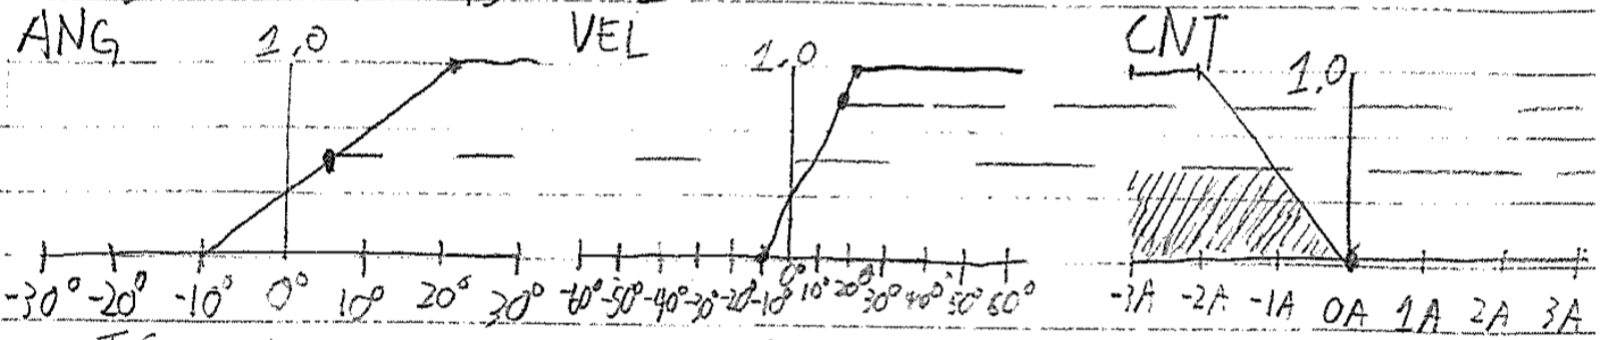
\includegraphics[scale=0.5]{plplnl.png}\\
If ANG is PL and VEL is NL, then CNT is NC\\
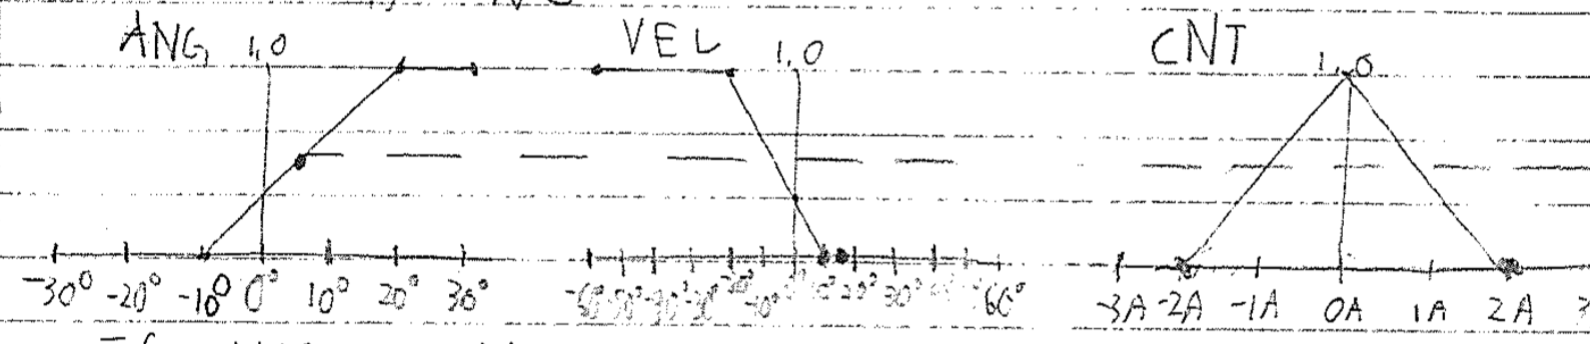
\includegraphics[scale=0.5]{plnlnc.png}\\
If ANG is NL and VEL is PL, then CNT is NC\\
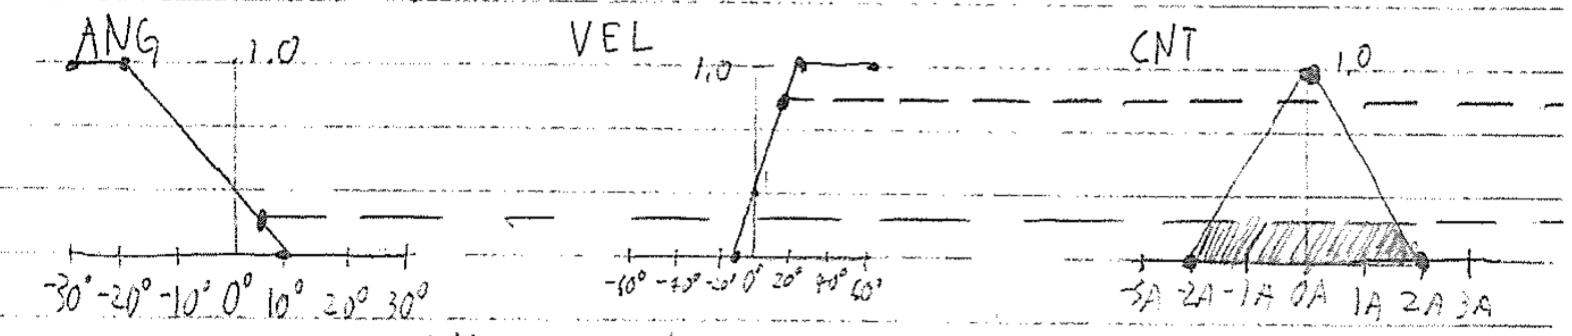
\includegraphics[scale=0.5]{nlplnc.png}\\
If ANG is NL and VEL is NL, then CNT is PL\\
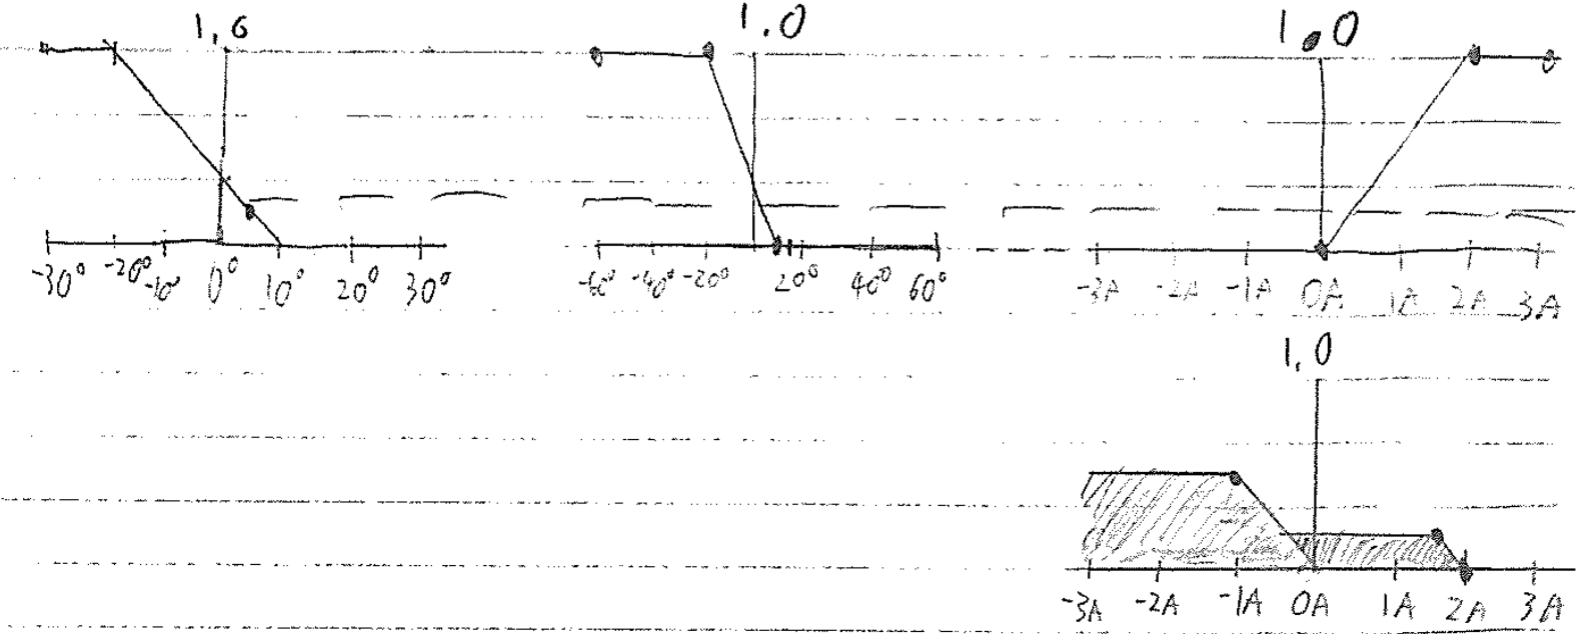
\includegraphics[scale=0.5]{rest.png}\\

\pagebreak

\section*{Question 2}

Case B, overlapped membership functions, provides more realistic control than case A for several reasons. If the temperature is close to PL, it is desirable to start increasing the cooler. However, as seen in the figure, the case A, where membership functions are not overlapped, does not do so. Therefore, case B seems to provide more realistic control inferences.

\pagebreak

\section*{Question 3}

$\mu_R$(x,y,z) = $max_i(\mu_{Ri} + \alpha_i * \mu_{Ri} (1-\mu_{Ri}))$ \\
= $max_i(\mu_{Ri} * (1 + \alpha_i * (1-\mu_{Ri}))$
\\\\
As can be seen, $\alpha_i$ is the enhancing factor. $0 \le \mu_{Ri} \le 1$, and $0 \le 1-\mu_{Ri} \le 1$. It means that depending on the $\alpha_i$ value, the element's value at changes. If $\alpha_i > 0$, the value of the element i increases. If $\alpha_i < 0$, the value of the element i decreases. As seen in the cases, $\alpha_i$ offers the weight to the rule-based decision making process. if $\alpha_i > 0$, such decision will be mare likely to be chosen at i, for the decision process finds the max. if $\alpha_i < 0$, the decision is less likely to be chosen, for the value at i decreases.

\pagebreak

\section*{Question 4}

\subsection*{I)}
\subparagraph*{(a)}
Servo control of a single axis positioning table with a permanent magnet DC motor is a linear system. It is recommended to use Sugeno fuzzy model because it is fairly simple system with one control variable.
\subparagraph*{(b)}
Active control of a vehicle suspension system is multivariable linear system. Sugeno model can handle multivariable linear system. It is recommended to use Sugeno model, since the output can be modelled.
\subparagraph*{(c)}
Control of a rotary cement kiln is nonlinear and complex system that is also difficult to model. Since it is non-linear and hard to model, Sugeno model is not recommended. In this case, Mamdani fuzzy model works fine, because it outputs the state.

\subsection*{II)}
\includegraphics[scale=0.2]{4II.png}\\
The crisp value of control action is 72.7gal/min after centeroid calculation. It is both RD and MN. It is sustainable, for the fuel usage is not that great.

\pagebreak

\section*{Question 5}
Please refer to the next page.
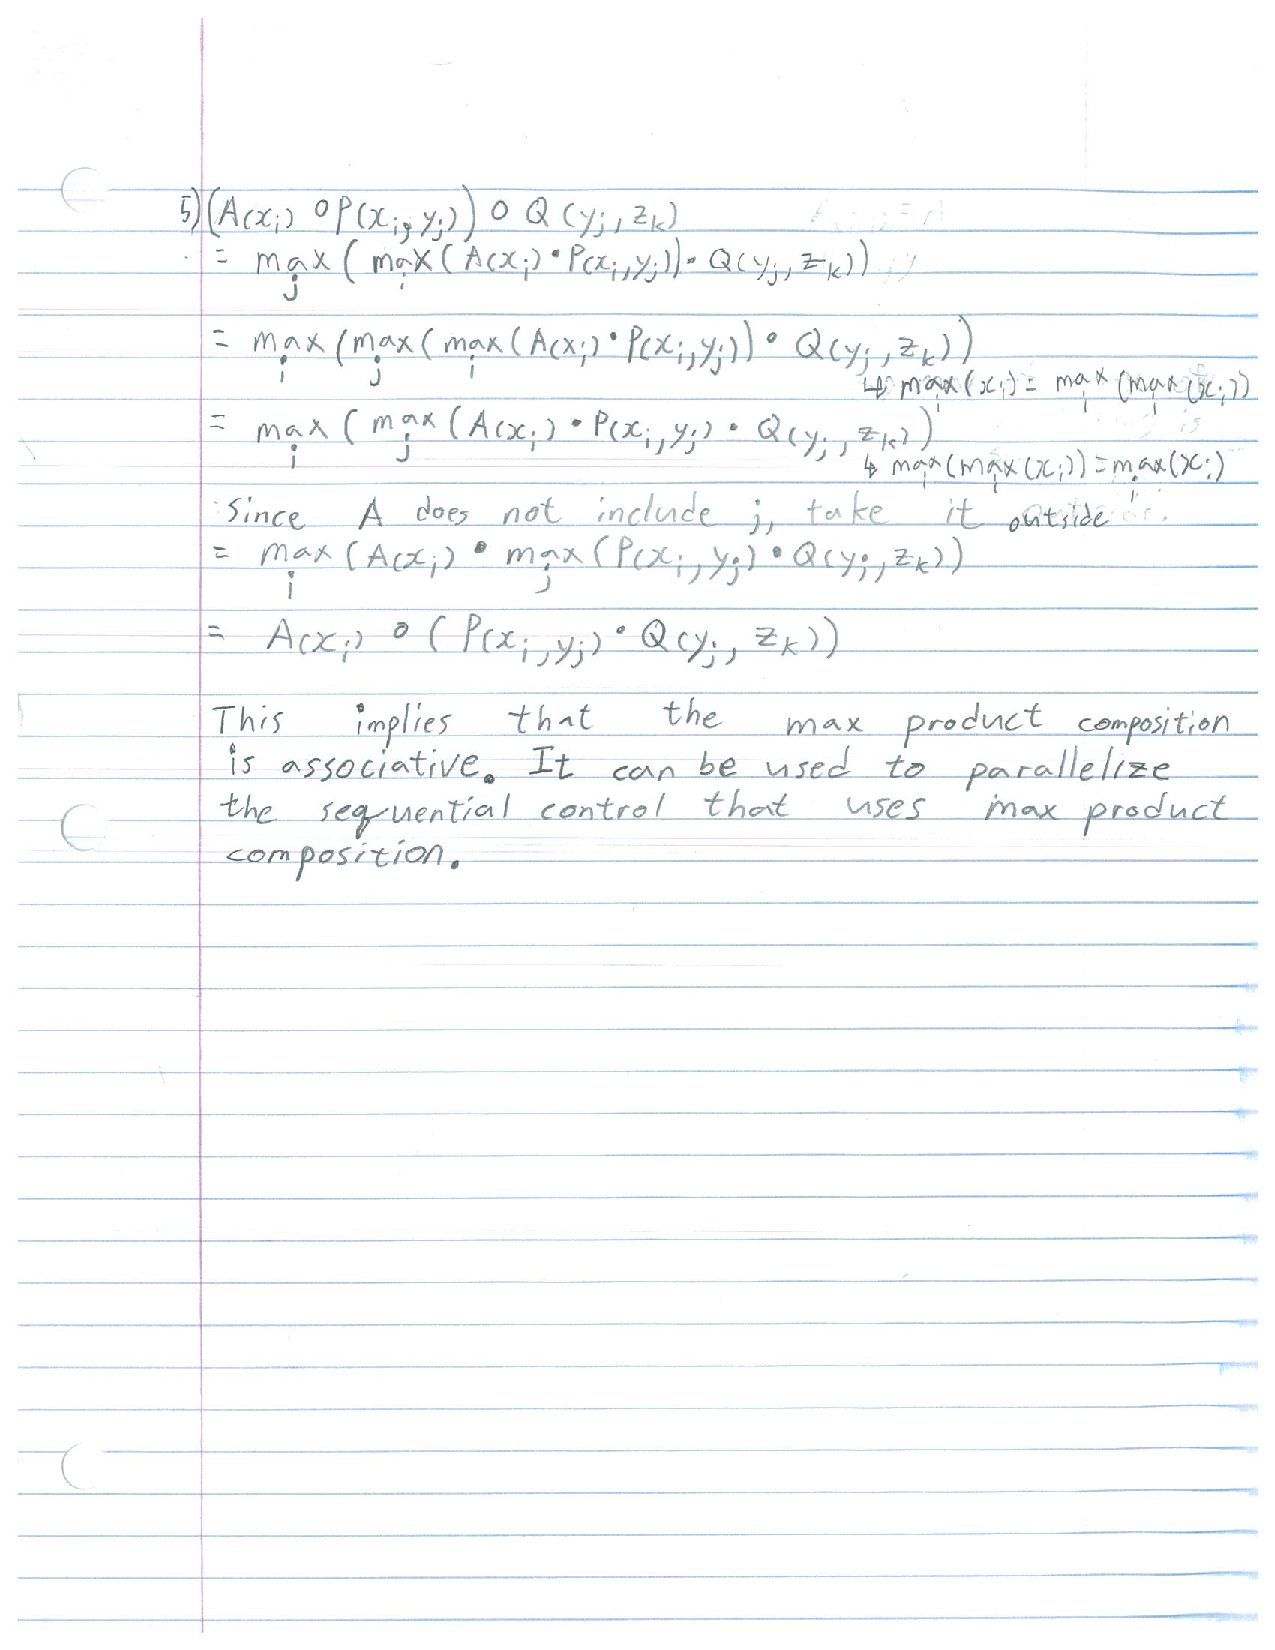
\includepdf[]{5.pdf}

\pagebreak


\end{document}